\documentclass[10pt,a4paper]{report}
\usepackage[utf8]{inputenc}
\usepackage{amsmath}
\usepackage{amsfonts}
\usepackage{amssymb}
\usepackage{float}
\usepackage{graphicx}
\graphicspath{{./images/}}
\usepackage{mathtools}
\DeclarePairedDelimiter\abs{\lvert}{\rvert}
\usepackage[left=3.00cm, right=3.00cm, top=3.00cm, bottom=3.00cm]{geometry}
\author{Del Prete Giovanni, Ghilardi Nicola, Polver Marco}
\title{BookSales UniBG: iterazione 1}

\begin{document}
	
	\maketitle
	\tableofcontents
	
	\section{Casi d'uso coperti}
	Di seguito vengono riportati i casi d'uso coperti dal software realizzato nell'iterazione 1:
	\begin{enumerate}
		\item UCS1: Registrazione studente
		\item UCS2: Login studente
		\item Logout
		\item UCS12: Ricerca studente
		\item UCS11: Ricerca annuncio
	\end{enumerate}
	Per l'implementazione di queste funzionalità si sono resi necessari due ulteriori passi:
	\begin{enumerate}
		\item \textit{Realizzazione dei modelli dei dati}: in Django i modelli sono delle classi Python che rappresentano le tabelle che devono essere realizzate all'interno del database.
		\item \textit{Realizzazione di uno script Python per il riempimento del database}: questo passo si è reso necessario per poter avere un numero consistente di dati su cui testare le diverse funzionalità dell'applicazione.
	\end{enumerate}

	\section{Note sul processo di implementazione}
	L'obiettivo iniziale era quello di realizzare questo progetto tramite un processo di Test Driven Development puro, tuttavia è stato necessario modificare questo processo permettendoci di testare alcune componenti del software solo dopo la loro implementazione. \\
	Questo va contro i principi del TDD, per cui bisognerebbe prima ideare una serie di test e solo dopo realizzare un codice sufficiente per passarli, ma si è reso necessario per due motivi:
	\begin{enumerate}
		\item \textit{Il nostro progetto è una applicazione web}: il testing delle applicazioni web risulta essere diverso rispetto al testing di applicazioni desktop e a volte i test risultano difficili anche solo da pensare prima di un'implementazione anche solo parziale della funzionalità da testare.
		\item \textit{Inesperienza con Django}: per tutti e tre questo progetto ha rappresentato l'occasione di provare Django per la prima volta. Questo framework è stato scelto in quanto particolarmente utilizzato al giorno d'oggi, ma nessuno di noi l'aveva utilizzato prima di questo progetto. Questo ha reso difficile, soprattutto all'inizio, l'applicazione del TDD, in quanto la realizzazione di un test presuppone una buona conoscenza degli strumenti utilizzati. I risultati ottenuti, tuttavia, sono ottimi e anche la nostra confidenza nell'utilizzo di Django è cresciuta notevolmente con il tempo.
	\end{enumerate}

	\subsection{Note sui test effettuati}
	Per la realizzazione dei test sono stati utilizzati due strumenti:
	\begin{itemize}
		\item La classe \textit{TestCase} fornita da Django, utilizzata per l'esecuzione di test strutturali.
		\item \textit{Selenium WebDriver}, una famosa API che permette di automatizzare l'utilizzo di un qualsiasi browser, molto utile per l'esecuzione di test funzionali.
	\end{itemize}
	\subsubsection{Test strutturali}
	Come già è stato detto in precedenza, i test strutturali sono stati effettuati utilizzando la classe TestCse che viene fornita da Django. \\
	L'esecuzione di test all'interno del framework Django risulta particolarmente comoda in quanto permette di utilizzare un vero e proprio "database di test", evitando quindi di sporcare il database normalmnte utilizzato dall'applicazione con dati utili solo in fase di test. \\
	I test strutturali effettuati per le varie funzionalità dell'applicazione verificano in genere i seguenti punti:
	\begin{itemize}
		\item Utilizzo del template HTML corretto in ogni pagina.
		\item Restituzione dello status code corretto (quasi sempre 200 o 404) a fronte della richiesta di una pagina web con determinati dati.
		\item Comportamento corretto dell'applicazione a seguito della somministrazione di dati corretti ed errati.
	\end{itemize}

	\subsubsection{Test funzionali}
	In uno script Python è stato utilizzato Selenium WebDriver per effettuare test funzionali. \\
	Le differenze tra i test che si possono eseguire con la classe TestCase e con il WebDriver sono notevoli:
	\begin{itemize}
		\item TestCase facilita l'utilizzo di richieste GET e POST. Selenium WebDriver è invece un puro sostituto dell'uomo, pertanto va istruito su quali tasti cliccare, i testi da inserire nelle varie textbox, ecc.
		\item Selenium WebDriver non fa parte del framework Django, pertanto le azioni compiute da esso andranno a scrivere nuovi dati nel vero database dell'applicazione e non in un database di prova.
	\end{itemize}
	I test funzionali sono stati realizzati basandosi sui \textit{casi d'uso}, pertanto non testano una singola funzionalità dell'applicazione ma la successione delle azioni compiute normalmente da un utente con un certo fine.
	
	\subsubsection{Copertura}
	Solo in poche occasioni la copertura dei test sui file Python presenti all'interno dell'applicazione risulta essere del 100\%, questo a causa dei seguenti motivi:
	\begin{itemize}
		\item All'interno dei file di un'app Django sono spesso presenti porzioni di codice di default che potrebbero non essere coperte.
		\item Alcune funzioni utilizzano la libreria "random", la quale rende il comportamento di alcune porzioni di codice imprevedibile; non è quindi possibile avere una copertura del 100\% in certe funzioni.
	\end{itemize}

	\section{L'architettura software}
	Trattandosi di una applicazione web realizzata con Django, l'architettura software è imposta dal framework utilizzato, pertanto sia in questa iterazione che nella successiva l'architettura non è cambiata. Il pattern utilizzato è il MVT già mostrato nell'iterazione 0. \\
	In questa iterazione sono stati sviluppati i 3 componenti di tale pattern.
	\section{Realizzazione dei modelli dei dati}
	Non tutte le tabelle progettate nella iterazione 0 sono state tradotte in modelli, in quanto solo una parte delle funzionalità del progetto sono state e saranno implementate, rendendo alcune tabelle superflue. 
	\begin{figure}[H]
		\centering
		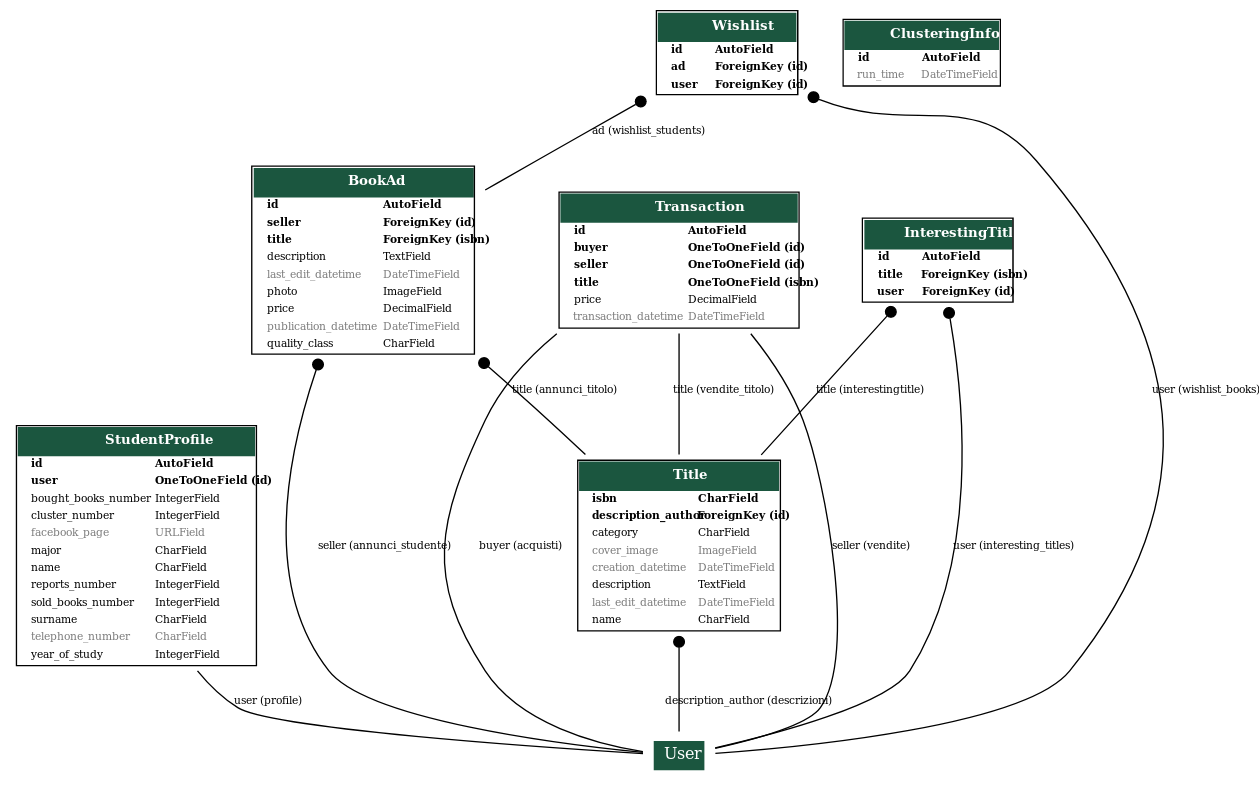
\includegraphics[height=10cm, width=17cm, keepaspectratio]{images/models.png}
		\caption{Diagramma dei modelli implementati}
	\end{figure}
	I modelli creati sono i seguenti:
	\begin{itemize}
		\item User: modello base fornito di default da Django. 
		\item StudentProfile: modello che si lega a User per fornire ulteriori informazioni sul singolo utente. I suoi campi:
		\begin{itemize}
			\item user: OneToOneField (simile a Foreign Key) che lega un solo User ad uno StudentProfile.
			\item name: nome dello studente.
			\item surname: cognome dello studente.
			\item telephone\_number: numero di telefono dello studente.
			\item facebook\_page: link alla pagina Facebook dello studente.
			\item major: corso di laurea a cui lo studente è iscritto.
			\item year\_of\_study: anno di corso.
			\item sold\_books\_number: numero di libri venduti.
			\item bought\_books\_number: numero di libri acquistati.
			\item reports\_number: numero di segnalazioni ricevute.
			\item cluster\_number: numero del cluster cui appartiene.
		\end{itemize}
		\item Title: modello per i singoli titoli. I campi sono:
			\begin{itemize}
				\item isbn: ISBN del titolo.
				\item name: nome del titolo.
				\item cover\_image: ImageField per l'immagine della copertina.
				\item description: descrizione scritta da un utente.
				\item description\_author: autore della descrizione.
				\item creation\_datetime: data di creazione del titolo nel database.
				\item last\_edit\_datetime: data dell'ultima modifica.
				\item category: categoria del titolo (fisica, matematica, informatica, meccanica, elettronica, economia, automazione, statistica).
			\end{itemize}
		\item BookAd: modello che descrive il singolo annuncio per la vendita di un libro. I campi sono:
			\begin{itemize}
				\item title: ForeignKey che lega un solo Title ad un BookAd.
				\item seller: ForeignKey che lega un solo User (il venditore) ad un BookAd.
				\item description: descrizione dell'annuncio.
				\item price: prezzo del libro.
				\item quality\_class: classe di qualità del libro (A, B, C, D).
				\item publication\_datetime: data di pubblicazione dell'annuncio.
				\item last\_edit\_datetime: data dell'ultima modifica dell'annuncio.
				\item photo: ImageField per una foto del libro.
			\end{itemize}
		\item Wishlist: modello che descrive l'appartenenza di un determinato annuncio alla wishlist di un utente. I campi sono:
			\begin{itemize}
				\item ad: ForeignKey che lega un oggetto di tipo Wishlist ad un solo BookAd, ovvero l'annuncio che fa parte della reale wishlist.
				\item user: ForeignKey che lega un oggetto di tipo Wishlist ad un solo utente.
			\end{itemize}
		\item InterestingTitle: modello che descrive l'appartenenza di un determinato titolo alla lista degli "interesting titles" di un utente. I campi sono:
			\begin{itemize}
				\item title: ForeignKey che lega un oggetto di tipo InterestingTitle ad un solo Title, ovvero l'annuncio che fa parte della reale lista "Interesting Titles".
				\item user: ForeignKey che lega un oggetto di tipo InterestingTitle ad un solo utente.
			\end{itemize}
		\item CluseringInfo: modello utilizzato per salvare le informazioni sull'esecuzione dell'algoritmo di clustering. I campi sono: 
			\begin{itemize}
				\item run\_time: data e ora della specifica esecuzione dell'algoritmo.
			\end{itemize}
	\end{itemize}
	I modelli sono stati testati tramite l'utilizzo dello script per il riempimento del database e indirettamente con i test effettuati su altre funzioni del sito web.
	
	\section{Realizzazione di uno script Python per il riempimento del database}
	Lo script crea i seguenti oggetti:
	\begin{itemize}
		\item 800 utenti e profili studente.
		\item 150 titoli.
		\item Un numero casuale tra 0 e 10 di "interesting titles" per ogni studente.
		\item Un numero casuale tra 10 e 50 di annunci per ogni titolo.
		\item Un numero casuale tra 0 e 20 di annunci nella wishlist dei singoli studenti.
	\end{itemize}

	\section{Implementazione delle altre funzionalità}
	
	\subsection{Template}
	Django mette a disposizione un vero e proprio linguaggio di programmazione utilizzabile all'interno dei template HTML e noi ne abbiamo fatto largo uso. \\
	E' inoltre possibile evitare di ripetere per ogni pagina web porzioni di codice HTML comune, estendendo un template comune contenente proprio quel codice da riutilizzare. \\
	
	Tutti i nostri template estendono il template "base.html", il quale descrive la barra di navigazione presente in tutto il sito web e la divisione tra titolo e corpo delle singole pagine web.
	
	\begin{figure}[H]
		\centering
		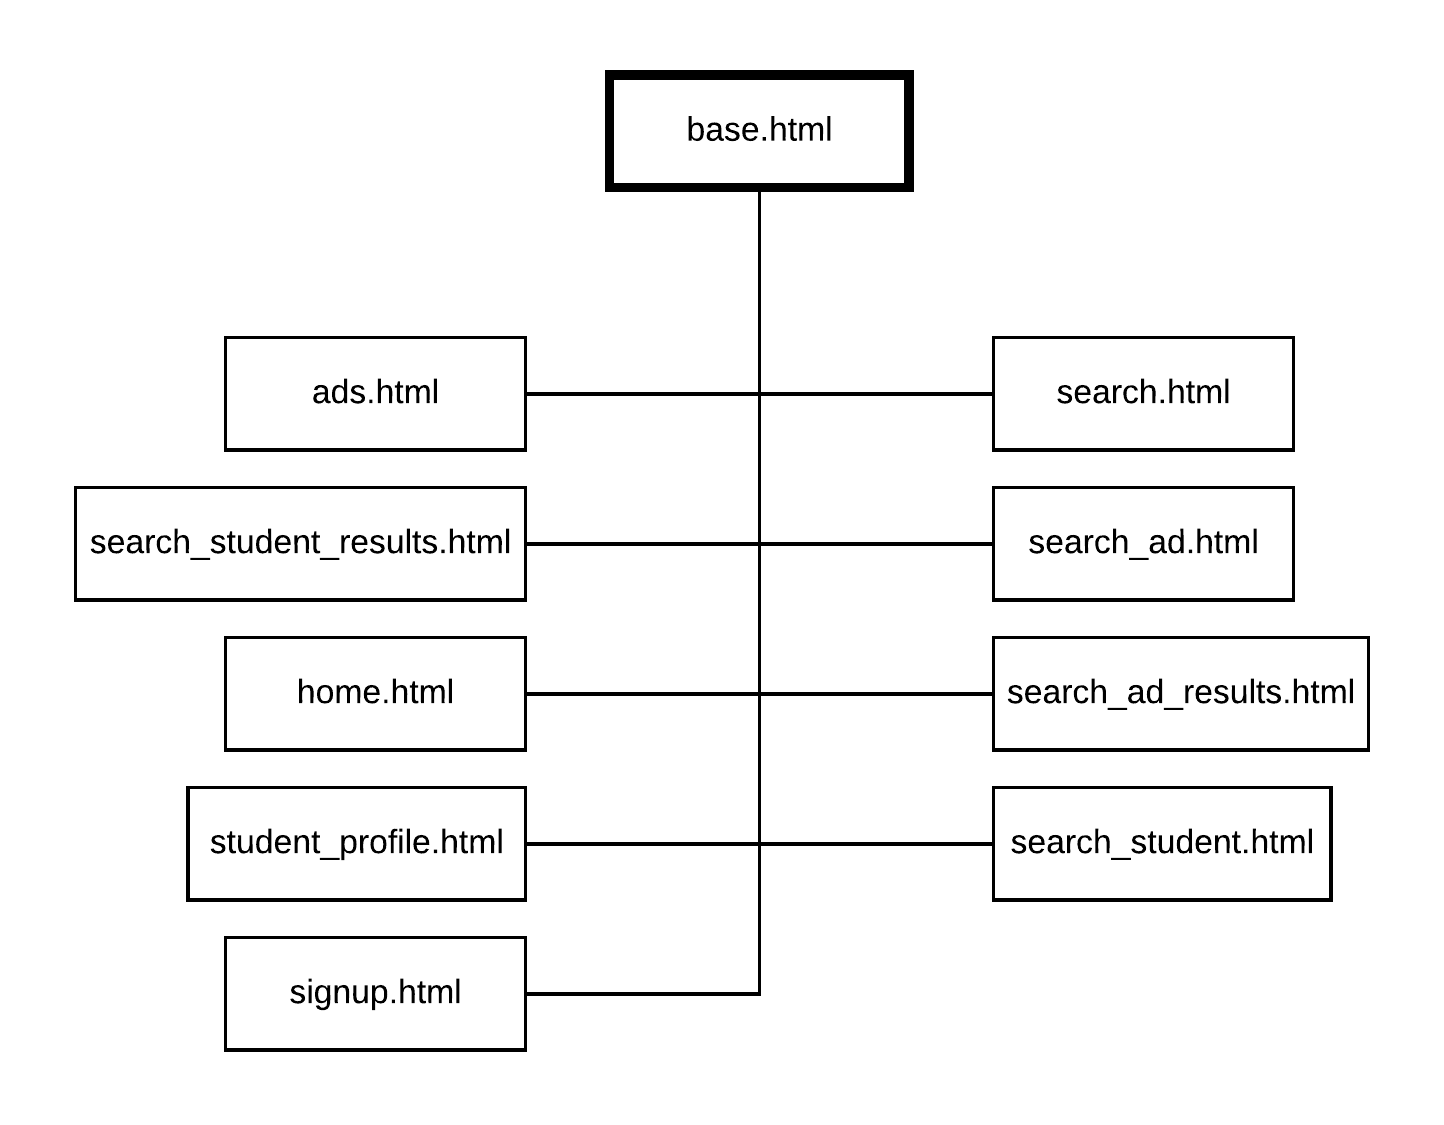
\includegraphics[height=10cm, width=17cm, keepaspectratio]{images/templates.png}
		\caption{Diagramma dei modelli implementati}
	\end{figure}
	
	\subsection{Login e logout}
	Il login e il logout sono stati implementati facilmente, in quanto è stato sufficiente utilizzare quelli già forniti da Django.
	
	\subsection{Registrazione di un nuovo utente}
	La registrazione di un nuovo utente implica implicitamente la creazione di un nuovo oggetto User e di un nuovo oggetto StudentProfile. Per questo motivo la pagina per la registrazione presenta due form, uno per la creazione dell'utente e uno per la creazione del profilo studente. \\
	I form sono stati realizzati da noi, così come il controllo sull'indirizzo email inserito (il quale deve appartenere al dominio unibg.it, coerentemente con le specifiche)
	
	
\end{document}